\documentclass[12pt,a4paper]{report}
\usepackage[utf8]{inputenc}
\usepackage[portuguese]{babel}
\usepackage{titlesec}
%\usepackage{lipsum}
\usepackage{graphicx}
\usepackage{float}
\usepackage{array}
\usepackage{multirow}
\usepackage{geometry}
 \geometry{
 a4paper,
 total={150mm,257mm},
 }


%\usepackage{minted}

\titleformat{\chapter}{\normalfont\huge}{\thechapter.}{10pt}{\huge}
\begin{document}
\begin{titlepage}
	
\includegraphics[width=0.2\textwidth]{UMEng.jpeg}\par\vspace{1cm}
	\begin{center}
		\Large\textbf{Desenvolvimento de Sistemas de Software}\vspace{2cm}
	\end{center}
	%{\scshape\LARGE Desenvolvimento de Sistemas de Software\par}\vspace{1cm}

	\date{}
	\textbf{Grupo de Trabalho:}
	\begin{table}[h]
		\centering
		\label{my-label}
		\begin{tabular}{lr}
		Ana Catarina Lopes Carvalho Sousa A78029 & 
\includegraphics[height=2cm]{Nacional.png} \\
		Ana Sofia Gomes Marques A75248           & 
\includegraphics[height=2cm]{Sofia.png}    \\
		Matias Nicolau Araújo A76234             & 
\includegraphics[height=2cm]{Matias.png}   \\
		Miguel Afonso Machado da Cunha A78478    & 
\includegraphics[height=2cm]{Miguel.png}   \\
		Pedro Mendes Félix da Costa A79003       & 
\includegraphics[height=2cm]{Mendes.png}   \\
		\end{tabular}
	\end{table}
	\vfill
	Mestrado Integrado em Engenharia Informática
\end{titlepage}
\tableofcontents
\chapter{Introdução}

Este relatório visa apresentar as decisões tomadas na realização da primeira fase do
trabalho prático da Unidade Curricular de Desenvolvimento de Sistemas de Software.
Procuramos justificar todas as considerações feitas na formulação do problema, na
elaboração do modelo de Domínio e de Use Cases.

Toda a modulação do problema e a apresentação neste relatório de diagramas,
esquemas e especificações, são feitas com recurso à linguagem de modelação UML,
abordada na UC.

O documento está estruturado em três capítulos. No primeiro é descrito o problema
e é feita uma proposta de modelo de domínio. São justificadas as inclusões de cada
entidade e dos relacionamentos entre elas, conforme os requisitos do problema. No
segundo capítulo são detalhados os atores do sistema que se consideraram, bem como a
especificação dos Use Cases de cada um. E por último, são apresentados os mockups, ou
seja, as propostas de interface.

\chapter{1. Modelo de domínio}
O sistema a implementar destina-se a suportar a configuração e gestão de turnos
práticos de um determinado curso.

Neste capítulo são apresentados os requisitos do problema e uma proposta de
modelo de Domínio.
\section{1.1. Descrição do modelo de Domínio}
O problema proposto é desenvolver um sistema de gestão de turnos práticos. Após
uma análise das necessidades e de factos reais, percebeu-se a existência dos seguintes
conceitos importantes na modulação do problema:

O Aluno, Turno, UC (Unidade Curricular), Trocas (de turno(s) que o aluno(a)
pretende efetuar), a Mudança (de turno), e as Faltas.

Tem-se que um Aluno frequenta 1 ou várias UC’s, cada UC possui 1 ou vários
turnos, 1 turno é frequentado por vários alunos, e consequentemente, 1 Aluno pode
frequentar 1 ou vários turnos, dependendo do número de UC’s que frequenta, e se estas
têm apenas aulas práticas/ práticas-laboratoriais ou se são constituídas por aulas
práticas/práticas-laboratoriais e aulas teóricas. Por exemplo se um aluno frequenta apenas
uma Unidade Curricular, este pode frequentar 1 ou dois turnos, dependendo das questões
levantadas acima, se este está inscrito a várias UC’s frequenta vários turnos.

Os turnos em que os alunos são alocados são previamente definidos pelo Diretor de
Curso, contudo o aluno pode efetuar várias trocas de turno, desde que encontre outro aluno
com quem efetuar essa troca, uma vez que cada turno tem um conjunto de dados,
constituído por um determinado no de vagas, um ou vários dias específicos em que é
lecionado e um determinado horário constituído por hora de início e hora de fim.

Por forma a efetivar as trocas, é necessário que o coordenador execute a respetiva
mudança de turno.

Associado a aluno temos o seu email de aluno, e o Nome, que o identificam. Ainda
no que diz respeito ao Aluno, este pode ser trabalhador estudante e nesse caso pode
efetuar as mudanças de turno que desejar, sem ter a necessidade de trocar com outro
aluno, desde que exista capacidade no turno que pretendem. A Capacidade depende da
sala em que o turno é lecionado e do tipo de turno, turnos práticos e práticos-laboratoriais,
têm limite máximo de alunos definido pelo coordenador da respetiva UC.

Existe ainda um sistema de faltas que é definido através de um relacionamento
ternário entre 1 docente que marca 0 ou várias faltas, o aluno que comete as faltas,
podendo estas ser 0 ou várias, e ainda o turno a que as faltas são cometidas, podendo ser
cometidas 0 ou várias faltas a cada turno.

\section{1.2 Modelo de Domínio}
\begin{figure}[H]
	\centering %optional
	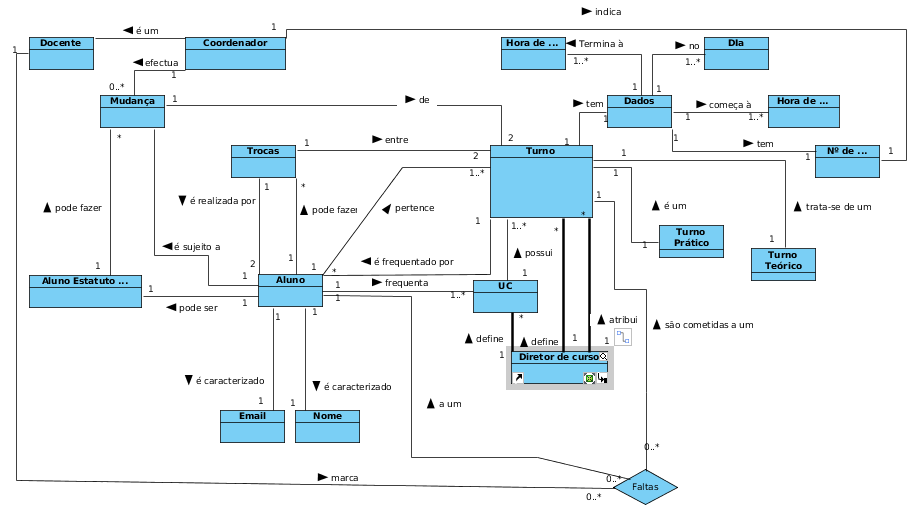
\includegraphics[width=\textwidth]{imgs/ModeloDominio.png}
	\caption{Modelo de Dominio}
\end{figure}

\chapter{2. Use Cases}
Para os \textit{Use Cases} foram considerados seis atores:
\begin{itemize}
	\item \textbf{Utilizador:} Todos os outros atores são utilizadores que necessitam de fazer o login para se autenticarem.
	\item \textbf{Aluno:} Responsável por escolher as UC’s que pretende frequentar e por solicitar o pedido troca de turno, assim como por aceitar sugestões de troca por parte de outros colegas. Este pode ainda consultar as UC’s e os turnos em que está inscrito.
	\item \textbf{Estatuto Especial:} É um aluno que pode também realizar trocas de turno sem precisar de trocar com outro colega.
	\item \textbf{Docente:} Responsável efetuar a marcação de presenças nos turnos que leciona. Pode também consultar as informações que dizem respeito aos turnos por ele lecionados.
	\item \textbf{Coordenador:} É o docente responsável pela UC, é responsável por efetuar as trocas de turnos tanto para alunos normais, como para alunos com estatuto especial, adicionando e removendo o aluno ao determinado turno.
	\item \textbf{Diretor de Curso:}Responsável por gerir as UC’s, os turnos e os alunos que os frequentam.
\end{itemize}
\section{2.1.1 Especificação dos Use Cases}
\subsection{2.1.1. Login}
O use case Login pertence ao Utilizador, e é o único use case que diz respeito a
todos os atores do sistema, e que consiste basicamente no processo de autenticação
necessário a cada utilizador para que possam interagir com o sistema.

O utilizador insere as suas credenciais e o sistema procede à validação das
mesmas, se estas forem válidas o utilizador fica autenticado, caso estas não sejam válidas
(exceção 1) o sistema informa o utilizador de que uma das credenciais que inseriu (email ou
password) não são válidas.

\begin{table}[h]
\centering
\caption{Login Use Case}
\label{usecase-login}
\begin{tabular}{|m{0.3\textwidth}|m{0.33\textwidth}|m{0.36\textwidth}|}
\hline
\multicolumn{3}{|l|}{Use Case: Login}                                                                                                                                                           \\ \hline
\multicolumn{3}{|l|}{Descrição: Utilizador efetua login}                                                                                                                                        \\ \hline
\multicolumn{3}{|l|}{Pré-condição: --}                                                                                                                                                          \\ \hline
\multicolumn{3}{|l|}{Pós-condição: Utilizador fica autenticado}                                                                                                                                 \\ \hline
                                                                                            & Ator                                        & Sistema                                             \\ \hline
\multirow{4}{*}{Comportamento Normal}                                                       & \multicolumn{1}{l|}{1. Inserir credenciais} &                                                     \\ \cline{2-3} 
                                                                                            &                                             & 1. Valida credenciais                               \\ \cline{2-3} 
                                                                                            &                                             & 2. Autentica                                        \\ \cline{2-3} 
                                                                                            &                                             & 3. Informa de sucesso                               \\ \hline
\begin{tabular}[c]{@{}l@{}}Exceção 1\\ {[}Credenciais Inválidas{]}\\ (passo 1)\end{tabular} &                                             & 1.1 Informa que o email ou password não são válidos \\ \hline
\end{tabular}
\end{table}
\subsection{2.1.2 Pedir Troca}
O use case Pedir Troca é efetuado pelo Aluno, sendo que para tal este tem de estar
autenticado e tem de ter turnos atribuídos, na qual este sugere uma troca de turno com
outro aluno, para tal este começa por indicar qual o turno para que pretende ir, e em
seguida o sistema verifica se não existe nenhuma sobreposição com outros turnos, e caso
isso não aconteça, informa que o pedido foi registado com sucesso.

Contudo pode acontecer que o turno indicado pelo aluno não exista, e nesse caso o
sistema informa que o turno não existe.

Como comportamento alternativo, caso ocorra sobreposição de turnos, o aluno pode
indicar que pretende continuar com o pedido, e neste caso o sistema regista o pedido.
Assim como o aluno, pode depois de o sistema verificar que existe sobreposição, optar por
não escolher o turno, e o sistema cancela o pedido.

\begin{table}[h]
\centering
\caption{My caption}
\label{my-label}
\begin{tabular}{|m{0.3\textwidth}|m{0.33\textwidth}|m{0.36\textwidth}|}
\hline
\multicolumn{3}{|m{\textwidth}|}{Use Case: Pedir troca}                                                                                                                                                                                            \\ \hline
\multicolumn{3}{|m{\textwidth}|}{Descrição: Utilizador pede para efetuar uma troca}                                                                                                                                                                \\ \hline
\multicolumn{3}{|m{\textwidth}|}{Pré-condição: O Utilizador está autenticado como Aluno, tem turnos atribuidos e o período de aulas ainda não começou.}                                                                                            \\ \hline
\multicolumn{3}{|m{\textwidth}|}{Pós-condição: Utilizador fica com um pedido de troca registado}                                                                                                                                                   \\ \hline
                                                                                                                                 & Ator                                            & Sistema                                           \\ \hline
\multirow{4}{*}{Comportamento Normal}                                                                                            & 1. O Aluno indica o turno para que pretende ir. &                                                   \\ \cline{2-3} 
                                                                                                                                 &                                                 & 2. Verifica se haverá sobreposição                \\ \cline{2-3} 
                                                                                                                                 &                                                 & 3. O sistema regista o pedido                     \\ \cline{2-3} 
                                                                                                                                 &                                                 & 4. Informa que o turno foi registado com sucesso. \\ \hline
\begin{tabular}[c]{@{}l@{}}Exceção 1\\ {[}Turno não existe{]}\\ (passo 2)\end{tabular}                                           &                                                 & 2.1 Informa que o turno não existe.               \\ \hline
\multirow{3}{*}{\begin{tabular}[c]{@{}l@{}}Alternativa 1\\ {[}Mudança impica sobreposição de turnos{]}\\ (passo 2)\end{tabular}} &                                                 & 2.1. Informa que o turno não existe.              \\ \cline{2-3} 
                                                                                                                                 & 2.2. Indica que queri pedir a troca na mesma.   &                                                   \\ \cline{2-3} 
                                                                                                                                 &                                                 & 2.3. Regressa ao passo 3.                         \\ \hline
\begin{tabular}[c]{@{}l@{}}Exceção 2\\ {[}Não quer pedir o turno{]}\\ (passo 2.2)\end{tabular}                                   &                                                 & 2.2.1 Informa que o pedido foi cancelado.         \\ \hline
\end{tabular}
\end{table}


\chapter{trash}
\emph{text}
\textit{textit}
\textbf{textbf}
\small text
\large text
\huge text
\small
%\newpage
%\par
%\noindent
%\vspace{}
%\hspance{}
%\\
%slides.com/dinispeixoto/deck

1+1

$1+1$

$$ a+b $$

$$\sum_{i=1}^{10} t_i $$

%www.tablegenerator.com

\begin{itemize}
	\item The individual entries are indicated with a black do, a so-called bullet.
	\item cenas
\end{itemize}

\section{First Section}
\subsection{First subsection}
\subsubsection{First subsubsection}
\chapter{Second chapter}

%\input{code.tex}

\chapter{Third chapter}
\end{document}





